

%---------------------------------------------------

\newpage

\section{Urban Morphogenesis by Aggregation-diffusion}{Morphogenèse Urbaine par Agrégation-diffusion}

\label{sec:densitygeneration}


%---------------------------------------------------



\bpar{
We study a stochastic model of urban growth generating spatial distributions of population densities at an intermediate mesoscopic scale. The model is based on the antagonist interplay between the two opposite abstract processes of aggregation (preferential attachment) and diffusion (urban sprawl). Introducing indicators to quantify precisely urban form, the model is first statistically validated and intensively explored to understand its complex behavior across the parameter space. We then compute real morphological measures on local areas of size 50km covering all European Union, and show that the model can reproduce most of existing urban morphologies in Europe. It implies that the morphological dimension of urban growth processes at this scale are sufficiently captured by the two abstract processes of aggregation and diffusion.
}{
Nous étudions un modèle stochastique de croissance urbain générant des distribution spatiales de densité de population à une échelle intermédiaire mesoscopique. Le modèle se base sur le jeu antagoniste entre les deux processus abstrait opposé de l'agrégation (attachement préférentiel) et de la diffusion (étalement urbain). En utilisant des indicateurs pour quantifier précisément la forme urbaine, le modèle est d'abord validé statistiquement puis exploré intensivement pour comprendre son comportement complexe sur son espace de paramètres. Ayant calculé précédemment les mesures morphologiques réelles sur des aires locales de taille 50km couvrant l'ensemble de l'Union Européenne, nous les utilisons pour montrer que le modèle peut reproduire la plupart des morphologies urbaines existantes en Europe. Cela implique que la dimension morphologique des processus de croissance urbaine à cette échelle est capturée de manière suffisante par les deux processus abstraits d'agrégation et de diffusion.
}


\subsection{Context}{Contexte}


\bpar{
The study of urban growth, and more particularly its quantification, is more than ever a crucial issue in a context where most of the world population live in cities which expansion has significant environmental impacts~\cite{seto2012global} and that have therefore to ensure an increased sustainability and resilience to climate change. The understanding of drivers for urban growth can lead to better integrated policies. It is however a question far from being solved in the diverse related disciplines: Urban Systems are complex socio-technical systems that can be studied from a large variety of viewpoints. Batty has advocated in that sense for the construction of a dedicated science defined by its objects of study more than the methods used~\cite{batty2013new}, what would allow easier coupling of approaches and therefore Urban Growth models taking into account heterogeneous processes. The processes that a model can grasp are also linked to the choice of the scale of study. At a macroscopic scale, models of growth in system of cities are mainly the concern of economics and geography. \cite{gabaix1999zipf} shows that in first approximation, the Gibrat's model postulating random growth rates not depending on city size, yield the well-know Zipf's law, or rank-size law, which is a typical stylized fact witnessing hierarchy in systems of cities. It was however shown empirically that systematic deviations to this law exist~\cite{rozenfeld2008laws}, and that spatial interactions may be responsible for it. Models integrating spatial interactions include for example \cite{bretagnolle2000long} that introduces a growth model in which these interactions, that are function of distance and the geography, play a significant role in growth rates. More recently, \cite{favaro2011gibrat} has extended this model by taking into account innovation waves between cities as a driver. The interplay of space, economic and population growth is studied by the Marius model~\cite{cottineau2014evolution} in the case of the former Soviet Union, on which model performance is shown improved compared to models without interactions.
}{
L'étude de la croissance urbaine, et plus particulièrement sa quantification, est plus que jamais un enjeu crucial dans un contexte ou la majorité de la population mondiale vit dans des villes dont l'expansion a des impacts environnementaux significatifs~\cite{seto2012global} et qui doivent pour cela assurer une soutenabilité et une résilience au changement climatique accrues. La compréhension des moteurs de la croissance urbaine devrait conduire à l'élaboration de politiques mieux intégrées. Il s'agit cependant d'une question loin d'être résolue dans les diverses disciplines concernées: les systèmes urbains sont des systèmes socio-techniques complexes qui peuvent être étudiés d'une grande variété de points de vue. \noun{Batty} défend en ce sens la construction d'une science dédiée définie par ses objets d'étude plus que par les méthodes utilisées~\cite{batty2013new}, ce qui devrait permettre des couplages plus faciles entre approches et donc des modèles de croissance urbaine prenant en compte des processus hétérogènes. Les processus qu'un modèle peut prendre en compte sont également liés au choix de l'échelle d'étude. A une échelle macroscopique, les modèles de croissance pour les systèmes de villes sont majoritairement le sujet de l'économie et de la géographie. \cite{gabaix1999zipf} montre qu'en première approximation, le modèle de Gibrat postulant des taux de croissance aléatoires ne dépendant pas de la taille des villes, produit la bien connue loi de Zipf, ou loi rang-taille, qui est un fait stylisé typique témoignant d'une hiérarchie dans les systèmes de villes. Il a cependant été démontré empiriquement que des déviations systématiques à cette loi existent~\cite{rozenfeld2008laws}, et que les interactions spatiales pourraient en être responsables. Les modèles intégrant les interactions spatiales incluent par exemple \cite{bretagnolle2000long} qui introduit un modèle de croissance dans lequel ces interactions, qui sont fonction de la distance et de la géographie, jouent un rôle significatif dans les taux de croissance. Plus récemment, \cite{favaro2011gibrat} a étendu ce modèle en prenant en compte les vagues d'innovation entre les villes comme facteur d'influence. Les relations entre espace, croissance économique et croissance de la population sont étudiées par le modèle Marius~\cite{cottineau2014evolution} pour le cas de l'ex-Union Soviétique, pour lequel la performance du modèle est démontrée améliorée par rapport aux modèles sans interactions.
}

\bpar{
At smaller scales, that can be understood as microscopic or mesoscopic depending on the resolution and extent of models, agents of models fundamentally differ. Space is generally taken into account in a finer way, through neighborhood effects for example. For example, \cite{andersson2002urban} propose a micro-based model of urban growth, with the purpose to replace non-interpretable physical mechanisms with agent mechanisms, including interactions forces and mobility choices. Local correlations are used in \cite{makse1998modeling}, which develops the model introduced in~\cite{makse1995modelling}, to modulate growth patterns to ressemble real configurations. The world of Cellular Automata (CA) models of Urban Growth~\cite{batty1994cells} also offers numerous examples. \cite{GEAN:GEAN940} introduced a generic framework for CA with multiple land use, based on local evolution rules. A model with simpler states (occupied or not) but taking into account global constraints is studied by \cite{ward2000stochastically}. The Sleuth model, initially introduced by \cite{clarke1998loose} for the San Francisco Bay area, and for which an overview of diverse applications is given in~\cite{clarke2007decade}, was calibrated on areas all over the world, yielding comparative measures through the calibrated parameters.
}{
A de plus petites échelles, qui peuvent être comprises comme microscopiques ou mesoscopiques selon la résolution et l'étendue spatiale des modèles, les agents des modèles diffèrent fondamentalement. L'espace est généralement pris en compte de manière plus fine, par les effets de voisinage par exemple. Par exemple, \cite{andersson2002urban} un modèle de croissance urbaine basé sur le microscopique, dans le but de remplacer des mécanismes physiques non interprétables par des mécanismes d'agents, incluant des forces d'interaction et des choix de mobilité. Les corrélations locales sont utilisées par \cite{makse1998modeling}, qui développe le modèle introduit dans \cite{makse1995modelling}, pour moduler les motifs de croissance pour qu'ils ressemblent à des configurations réelles. Le monde des modèles de croissance urbaine à automates cellulaires (CA)~\cite{batty1994cells} offre aussi de nombreux exemples. \cite{GEAN:GEAN940} introduit un cadre générique pour les CA avec usage du sol multiple, basé sur des règles d'évolution locales. Un modèle avec des états plus simples (occupé ou non) mais prenant en compte des contraintes globales est étudié par~\cite{ward2000stochastically}. Le modèle Sleuth, introduit initialement par~\cite{clarke1998loose} pour la zone de la Baie de San Francisco, et pour lequel un aperçu des diverses applications est donné dans~\cite{clarke2007decade}, a été calibré sur des régions tout autour du monde, fournissant des mesures comparatives au travers des paramètres calibrés.
}


\bpar{
Closely related to CA models but not exactly similar are Urban Morphogenesis models, which aim to simulate the growth of urban form from autonomous rules. \cite{frankhauser1998fractal} suggested that the fractal nature of cities is closely linked to the emergence of the form from the microscopic socio-economic interactions, namely urban morphogenesis. \cite{courtat2011mathematics} develops a morphogenesis model for urban roads alone, with growth rules based on geometrical considerations. These are shown sufficient to produce a broad range of patterns analog to existing ones. Similarly, \cite{raimbault2014hybrid} couples a CA with an evolving network to reproduce stylized urban form, from concentrated monocentric cities to sprawled suburbs. The Diffusion-Limited-Aggregation model, coming from physics, and which was first studied for cities by~\cite{batty1991generating}, can also be seen as a morphogenesis model. These kind of models, that sometimes can be classified as CA, have generally the particularity of being parsimonious in their structure.
}{
Assez proches des modèles CA, mais pas exactement similaires, sont les modèles de Morphogenèse Urbaine, qui visent à simuler la croissance de la forme urbaine à partir de règles autonomes. \cite{frankhauser1998fractal} suggère que la nature fractale des villes est en relation étroite avec l'émergence de la forme urbaine à partir des interactions socio-économiques microscopiques, à savoir la morphogenèse urbaine. \cite{courtat2011mathematics} développe un modèle de morphogenèse pour les routes urbaines seules, avec des règles de croissance basées sur des considérations géométriques. Celles ci sont montrées suffisantes pour produire un large spectre de motifs analogues à des existants. De manière similaire, \cite{raimbault2014hybrid} couple un CA avec un réseau évolutif pour reproduire des formes urbaines stylisées, de villes monocentriques concentrées à des banlieues étalées. Le modèle Diffusion-Limited-Aggregation, venant de la physique, et qui a été appliqué aux villes en premier par~\cite{batty1991generating}, peut aussi être vu comme un modèle de morphogenèse. Ce type de modèles, qui peuvent parfois être classifiés comme CA, ont généralement la particularité d'être parcimonieux dans leur structure. Des modèles similaires ont également été étudiés en biologie pour la diffusion de population par exemple~\cite{bosch1990velocity}.
}


\bpar{
We study in this section a morphogenesis model, at the mesoscopic scale, aimed at being simplistic in its rules and variables, but trying to be accurate in the reproduction of existing patterns. The underlying question is to explore the performance of simple mechanisms in reproducing complex urban patterns. We consider abstract processes, namely aggregation and diffusion, candidates as partially explanatory drivers of urban growth, based on population only, that will be detailed in model rationale below. An important aspect we introduce is the quantitative measure of urban form, based on a combination of morphological indicators, to quantify and compare model outputs and real urban patterns. Our contribution is significant on several points: (i) we compute local morphological characteristics on a large spatial extent (full European Union); (ii) we give significant insights into model behavior through extensive exploration of the parameter space; (iii) we show through calibration that the model is able to reproduce most of existing urban forms across Europe, and that these abstract processes are sufficient to explain urban form alone. The rest of this paper is organized as follows: we first describe formally the model and the morphological indicators. We then detail values of morphological measures on real data, study the behavior of the model by exploring its parameter space and through a semi-analytical approach to a simplified case, and we describe results of model calibration.
}{
Nous étudions dans cette section un modèle de morphogenèse, à l'échelle mesoscopique, dont le but est d'être simple dans ses règles et variables, mais visant à être performant pour la reproduction de motifs existants. La question sous-jacente est l'exploration de la performance de mécanismes simples pour reproduire des formes urbaines complexes. Nous considérons des processus abstrait, précisément l'agrégation et la diffusion, comme candidats comme facteurs potentiellement explicatifs de la croissance urbaine, basés sur la densité de population seule, qui seront détaillés ci-dessous. Un aspect important que nous utilisons est la mesure quantitative de la forme urbaine, basée sur une combinaison d'indicateurs morphologiques, pour quantifier et comparer les sorties de modèle et les formes urbaines réelles. Notre contribution est significative sur plusieurs points: (i) le calcul des caractéristiques morphologiques réelles sur une étendue spatiale conséquente (Union Européenne complète); (ii) nous apprenons le comportement du modèle par une exploration conséquente de l'espace des paramètres; (iii) nous montrons par la calibration que le modèle est capable de reproduire la majorité des formes urbaines existantes en Europe, et que ces processus abstraits sont suffisants pour expliquer la forme urbaine seule. La suite de cette section est organisée de la façon suivante : nous décrivons d'abord formellement le modèle. Nous étudions ensuite le comportement du modèle par une exploration de l'espace des paramètres et par une approche semi-analytique d'un cas simplifié, puis nous décrivons les résultats de la calibration du modèle.
}





\subsection{Model and Results}{Modèle et Résultats}



\subsubsection{Urban growth model}{Modèle de croissance urbaine}




%%%%%%%%%%%%%%%%%%%%%%%%
\paragraph{Rationale}{Rationelle}

\bpar{
Our model is based on widely accepted ideas of diffusion-aggregation processes for Urban Processes. The combination of attraction forces with repulsion, due for example to congestion, already yield a complex outcome that has been shown under some simplifying assumptions to be representative of urban growth processes. A model capturing these processes was introduced by~\cite{batty2006hierarchy}, as a cell-based variation of the DLA model~\cite{batty1991generating}. Indeed, the tension between antagonist aggregation and sprawl mechanisms may be an important process in urban morphogenesis. For example \cite{fujita1996economics} opposes centrifugal forces with centripetal forces in the equilibrium view of urban spatial systems, what is easily transferable to non-equilibrium systems in the framework of self-organized complexity: a urban structure is a far-from-equilibrium system that has been driven to this point by these opposite forces. The two contradictory processes of urban concentration and urban sprawl are captured by the model, what allows to reproduce with a good precision a large number of existing morphologies. We can expect aggregation mechanisms such as preferential attachment to be good candidates in urban growth explanation, as it was shown that the Simon model based on them generates power-laws typical of urban systems (scaling laws for example)~\cite{2016arXiv160806313S}. The question at which scale is it possible and relevant to define and try to simulate urban form is rather open, and will in fact depend on which issues are being tackled. Working in a typical setting of morphogenesis, the processes considered are local and our model must have a resolution at the micro-level. We however want to quantify urban form on consistent urban entities, and will work therefore on spatial extents of order 50$\sim$100km. We sum up these two aspects by stating that the model is at the \emph{mesoscopic scale}.
}{
Notre modèle est basé sur des idées largement acceptées de processus d'agrégation-diffusion pour les les processus urbains. La combinaison de forces d'attraction avec celles de répulsion, dues par exemple à la congestion, fournit déjà une issue complexe qui a été montrée représentative des processus de croissance urbaine sous certaines hypothèses simplificatrices. Un modèle capturant ces processus a été introduit dans~\cite{batty2006hierarchy}, comme une variation cellulaire du modèle DLA~\cite{batty1991generating}. En effet, la tension entre les mécanismes antagonistes d'agrégation et d'étalement peut être un processus important pour la morphogenèse urbaine. Par exemple, \cite{fujita1996economics} oppose les forces centrifuges aux forces centripètes dans une vision d'équilibre des systèmes urbains spatiaux, ce qui peut facilement être transféré aux systèmes hors équilibre dans le cadre de la complexité auto-organisée: une structure urbaine est un système \emph{far-from-equilibrium} qui a été conduit à ce point par ces forces opposées. Les deux processus contradictoires de concentration urbaine et d'étalement urbain sont capturés par le modèle, ce qui permet de reproduire avec une bonne précision un grand nombre de morphologies existantes. Nous pouvons supposer que des mécanismes d'agrégation comme l'attachement préférentiel sont des bons candidats pour expliquer la croissance urbaine, puisqu'il a été montré que le modèle de Simon qui se base dessus génère des \emph{power-law} qui sont typiques des systèmes urbains (lois d'échelles par exemple)~\cite{2016arXiv160806313S}. La question de l'échelle à laquelle il est possible et pertinent de définir et d'essayer de simuler la croissance urbaine est relativement ouverte, et dépendra en fait de quels problèmes sont considérés. Travaillant dans un cadre typique de la morphogenèse, les processus considérés sont locaux et notre modèle doit avoir une résolution au niveau microscopique. Nous voulons cependant quantifier la forme sur des unités urbaines cohérentes, et travaillerons ainsi sur des étendues spatiales d'ordre 50$\sim$100km. Nous résumons ces deux aspects en posant que le modèle est à l'échelle \emph{mesoscopique}.
}

\paragraph{Formalization}{Formalisation}

\bpar{
We formalize now the model and its parameters. The world is a square grid of width $N$, in which each cell is characterized by its population $(P_i(t))_{1\leq i\leq N^2}$. We consider the grid initially empty, i.e. $P_i(0)=0$, but the model can be easily generalized to any initial population distribution. The population distribution is updated in an iterative way. At each time step,
}{
Nous formalisons à présent le modèle et ses paramètres. Le monde est une grille carrée de côté $N$, dans lequel chaque cellule est caractérisée par sa population $(P_i(t))_{1\leq i\leq N^2}$. Nous considérons la grille initialement vide, i.e. $P_i(0)=0$, mais le modèle peut être facilement généralisé à n'importe quelle distribution initiale de population. La distribution de population est mise à jour de façon itérative. A chaque pas de temps,
}

\bpar{
\begin{enumerate}
\item Total population is increased by a fixed number $N_G$ (growth rate). Each population unit is attributed independently to a cell following a preferential attachment such that 
\begin{equation}
\Pb{P_i(t+1)=P_i(t)+1|P(t+1)=P(t)+1}=\frac{(P_i(t)/P(t))^{\alpha}}{\sum(P_i(t)/P(t))^{\alpha}}
\end{equation}
The attribution being uniformly drawn if all population are equal to 0.
\item A fraction $\beta$ of population is diffused to cell neighborhood (8 closest neighbors receiving each the same fraction of the diffused population). This operation is repeated $n_d$ times.
\end{enumerate}
}{
\begin{enumerate}
\item La population totale est augmentée par un nombre fixe $N_G$ (taux de croissance). Chaque unité de population est attribuée indépendamment à une cellule suivant un attachement préférentiel tel que
\begin{equation}
\Pb{P_i(t+1)=P_i(t)+1|P(t+1)=P(t)+1}=\frac{(P_i(t)/P(t))^{\alpha}}{\sum(P_i(t)/P(t))^{\alpha}}
\end{equation}
L'attribution est tirée de manière uniforme si toutes les populations sont égales à 0.
\item Une fraction $\beta$ de la population est diffusée au voisinage de chaque cellule (les 8 plus proches voisins recevant chacun la même fraction de la population diffusée). Cette opération est répétée $n_d$ fois.
\end{enumerate}
}

\bpar{
The model stops when total population reaches a fixed parameter $P_m$. To avoid bord effects such as reflecting diffusion waves, border cells diffuse their due proportion outside of the world, implying that the total population at time $t$ is strictly smaller than $N_G\cdot t$.
}{
Le modèle s'arrête que la population totale atteint un paramètre fixé $P_m$. Pour éviter les effets de bord comme des ondes de diffusion se réfléchissant, les cellules du bord diffusent la proportion qu'elles devraient hors du monde, ce qui implique que la population totale à l'instant $t$ est strictement plus petite que $N_G\cdot t$.
}

\bpar{
We summarize model parameters in Table~\ref{tab:density:parameters}, giving the associated processes and values ranges we use in the simulations. The total population of the area $P_m$ is exogenous, in the sense that it is supposed to depend on macro-scale growth patterns on long times. Growth rate $N_G$ captures both endogenous growth rate and migration balance within the area. The aggregation rate $\alpha$ sets the differences in attraction between cells, what can be understood as an abstract attraction coefficient following a scaling law of population. Finally, the two diffusion parameters are complementary since diffusing with strength $n_d\cdot \beta$ is different of diffusing $n_d$ times with strength $\beta$, the later giving flatter configuration.
}{
Nous résumons les paramètres du modèle dans la Table~\ref{tab:density:parameters}, donnant les processus associés et les bornes des valeurs utilisées dans les simulations. La population totale de la zone $P_m$ est exogène, au sens qu'elle est supposée dépendre de processus de croissance à l'échelle macroscopique sur le temps long. Le taux de croissance $N_G$ capture à la fois la croissance endogène et la balance migratoire dans la zone. Le taux d'agrégation $\alpha$ fixe la différence d'attractivité entre cellules, qui peut être interprétée comme un coefficient abstrait d'attraction suivant une loi d'échelle de la population. Enfin, les deux paramètres de diffusion sont complémentaires puisque diffuser avec force $n_d\cdot \beta$ est différent de diffuser $n_d$ fois avec force $\beta$, le dernier cas donnant des configurations plus plates.
}

% table summarizing parameters
%  $\alpha \in [0.1,4],\beta \in [0,0.5],n_d \in \{1,\ldots , 5\}, N_G \in [500,30000], P_m \in [1e4,1e6]$
%%%%%%%%%%%%%
\begin{table}[!ht]
\caption{{\bf Summary of model parameters.}}{\textbf{Résumé des paramètres}}\label{tab:density:parameters}
\begin{tabular}{|l|l|l|l|}
\hline
Parameter & Notation & Process & Range\\ \hline
Total population & $P_m$ & Macro-scale growth & $[1e4,1e6]$\\ \hline
Growth rate & $N_G$ & Meso-scale growth  & $[500,30000]$\\ \hline
Aggregation strength & $\alpha$ & Aggregation & $[0.1,4]$\\ \hline
Diffusion strength & $\beta$ & Diffusion & $[0,0.5]$\\ \hline
Diffusion steps & $n_d$ & Diffusion & $\{1,\ldots , 5\}$\\ \hline
\end{tabular}
\end{table}
%%%%%%%%%%%%%%


\paragraph{Measuring the Urban Form}{Mesure de la forme urbaine}

\bpar{
As our model is only density-based, we propose to quantify its outputs through spatial morphology, i.e. properties of the spatial distribution of density. At the scale chosen, these will be expected to translate various functional properties of the urban landscape. 
}{
Comme le modèle se base uniquement sur la densité, nous proposons de quantifier ses sorties par la morphologie spatiale, i.e. les propriétés de la distribution spatiale de la densité. A l'échelle choisie, on s'attend à ce qu'elle traduise diverse propriétés fonctionnelles de l'environnement urbain. Le contexte et la définition des indicateurs a déjà été donnée en section~\ref{sec:staticcorrelations}.
}


\subsubsection{Real data}{Données réelles}


Nous travaillons sur les valeur des indicateurs calculées en section~\ref{sec:staticcorrelations} pour l'Europe, sur les fenêtres de côté 50km avec résolution de 100 cellules. Nous posons donc pour la suite $N=100$ pour les simulations du modèle.





%%%%%%%%%%%%%%%%%%%%%%%%
\subsubsection*{Generation of urban patterns}{Génération de structures urbaines}


\paragraph{Implementation}{Implémentation}

\bpar{
The model is implemented both in NetLogo~\cite{wilensky1999netlogo} for exploration and visualization purposes, and in \texttt{Scala} for performance reasons and easy integration into OpenMole~\cite{reuillon2013openmole}, which allows a transparent access to High Performance Computing environments. Computation of indicator values on geographical data is done in \texttt{R} using the \texttt{raster} package~\cite{hijmans2015geographic}. Source code and results are available on the open repository of the project at \texttt{https://github.com/JusteRaimbault/Density}. Raw datasets for real indicator values and simulation results are available on Dataverse at \texttt{http://dx.doi.org/10.7910/DVN/WSUSBA}.
}{
Le modèle est implémenté à la fois en NetLogo~\cite{wilensky1999netlogo} pour des raisons d'exploration et de visualisation, et en \texttt{Scala} pour des raisons de performance et d'intégration plus aisée dans OpenMole~\cite{reuillon2013openmole}, qui permet un accès transparent aux environnements de calcul haute performance. Le calcul des valeurs des indicateurs sur les données géographiques est fait en \texttt{R} avec le package \texttt{raster}~\cite{hijmans2015geographic}. Le code source et les résultats sont disponibles sur le dépôt ouvert du projet\footnote{à \texttt{https://github.com/JusteRaimbault/Density}}. Les données des valeurs réelles des indicateurs et des résultats de simulation sont disponibles sur Dataverse\footnote{à \texttt{http://dx.doi.org/10.7910/DVN/WSUSBA}}. Nous avons dans le cadre de l'implémentation \texttt{Scala} implémenté la convolution de distribution en deux dimension par Transformée de Fourier rapide, permettant de transformer une complexité $O(N^4)$ en $O(N^2\log^2 N)$, puis implémenté les indicateurs qui ont pu être intégrés à une extension NetLogo dédiée~\ref{app:subsec:morphologyextension}.
}

\paragraph{Generated Shapes}{Formes générées}


\bpar{
The model has a relatively small number of parameters but is able to generate a large variety of shapes, extending beyond existing forms. In particular, its dynamical nature allows through the interplay between $P_m$ and $N_G$ parameter to choose between final configurations that can be non-stationary or semi-stationary, whereas the interplay between $\alpha$ and $\beta$ modulates the sprawl and the compactness of forms. We run the model for parameters varying in ranges given in Table~\ref{tab:parameters}, for a world size $N=100$. Fig.~\ref{fig:fig2} shows examples of the variety of generated shapes for different parameter values, with corresponding interpretations. The four very different shapes can be obtained with variation of a single parameter sometimes: going from a peri-urban area from a rural area implies an increased aggregation at the same level of diffusion. Note that the model is density driven, and that the parameter $P_m/N_G$ is what really influences the dynamics: the values of $P_m$ are in some cases not directly corresponding to the interpretations we made (for the rural in particular) that are done on densities. A rescaling keeps the settlement form and solves this issue. These examples show the potentiality of the model to produce diverse shapes. We need then to systematically tackle its stochasticity and explore its parameter space.
}{
Le modèle a un nombre relativement faible de paramètres mais est capable de générer une grande variété de formes, qui s'étendent au delà des formes existantes. Plus particulièrement, sa nature dynamique permet par la combinaison des paramètres $P_m$ et $N_G$ de choisir entre des configurations qui peuvent être non stationnaires ou semi stationnaires, tandis que l'interaction entre $\alpha$ et $\beta$ module l'étalement et le caractère compact des formes. Nous simulons le modèle pour des valeurs de paramètres variant dans les bornes données en Table~\ref{tab:density:parameters}, pour une taille de monde $N=100$. Fig.~\ref{fig:density:fig2} montre des exemples de la variété des formes urbaines générées pour différentes valeurs des paramètres, avec les interprétations correspondantes. Parmi les quatre formes très différentes, certaines peuvent être obtenues avec la variation d'un seul paramètre seulement : passer d'une zone péri-urbaine à une zone rurale implique une agrégation accrue au même niveau de diffusion. Il faut noter que le modèle est basé sur la densité, et que le paramètre $P_m/N_G$ est celui qui influence réellement la dynamique: les valeurs de $P_m$ ne correspondent dans certains cas pas directement aux interprétations qui en sont faites (pour le rural en particulier) qui sont faites sur les densités. Une homothétie garde la forme des établissements et résout ce problème. Ces exemples montrent la potentialité du modèle à produire des formes diverses. Nous devons ensuite étudier systématiquement sa stochasticité et explorer son espace des paramètres.
}


%%%%%%%%%%%%%
\begin{figure}
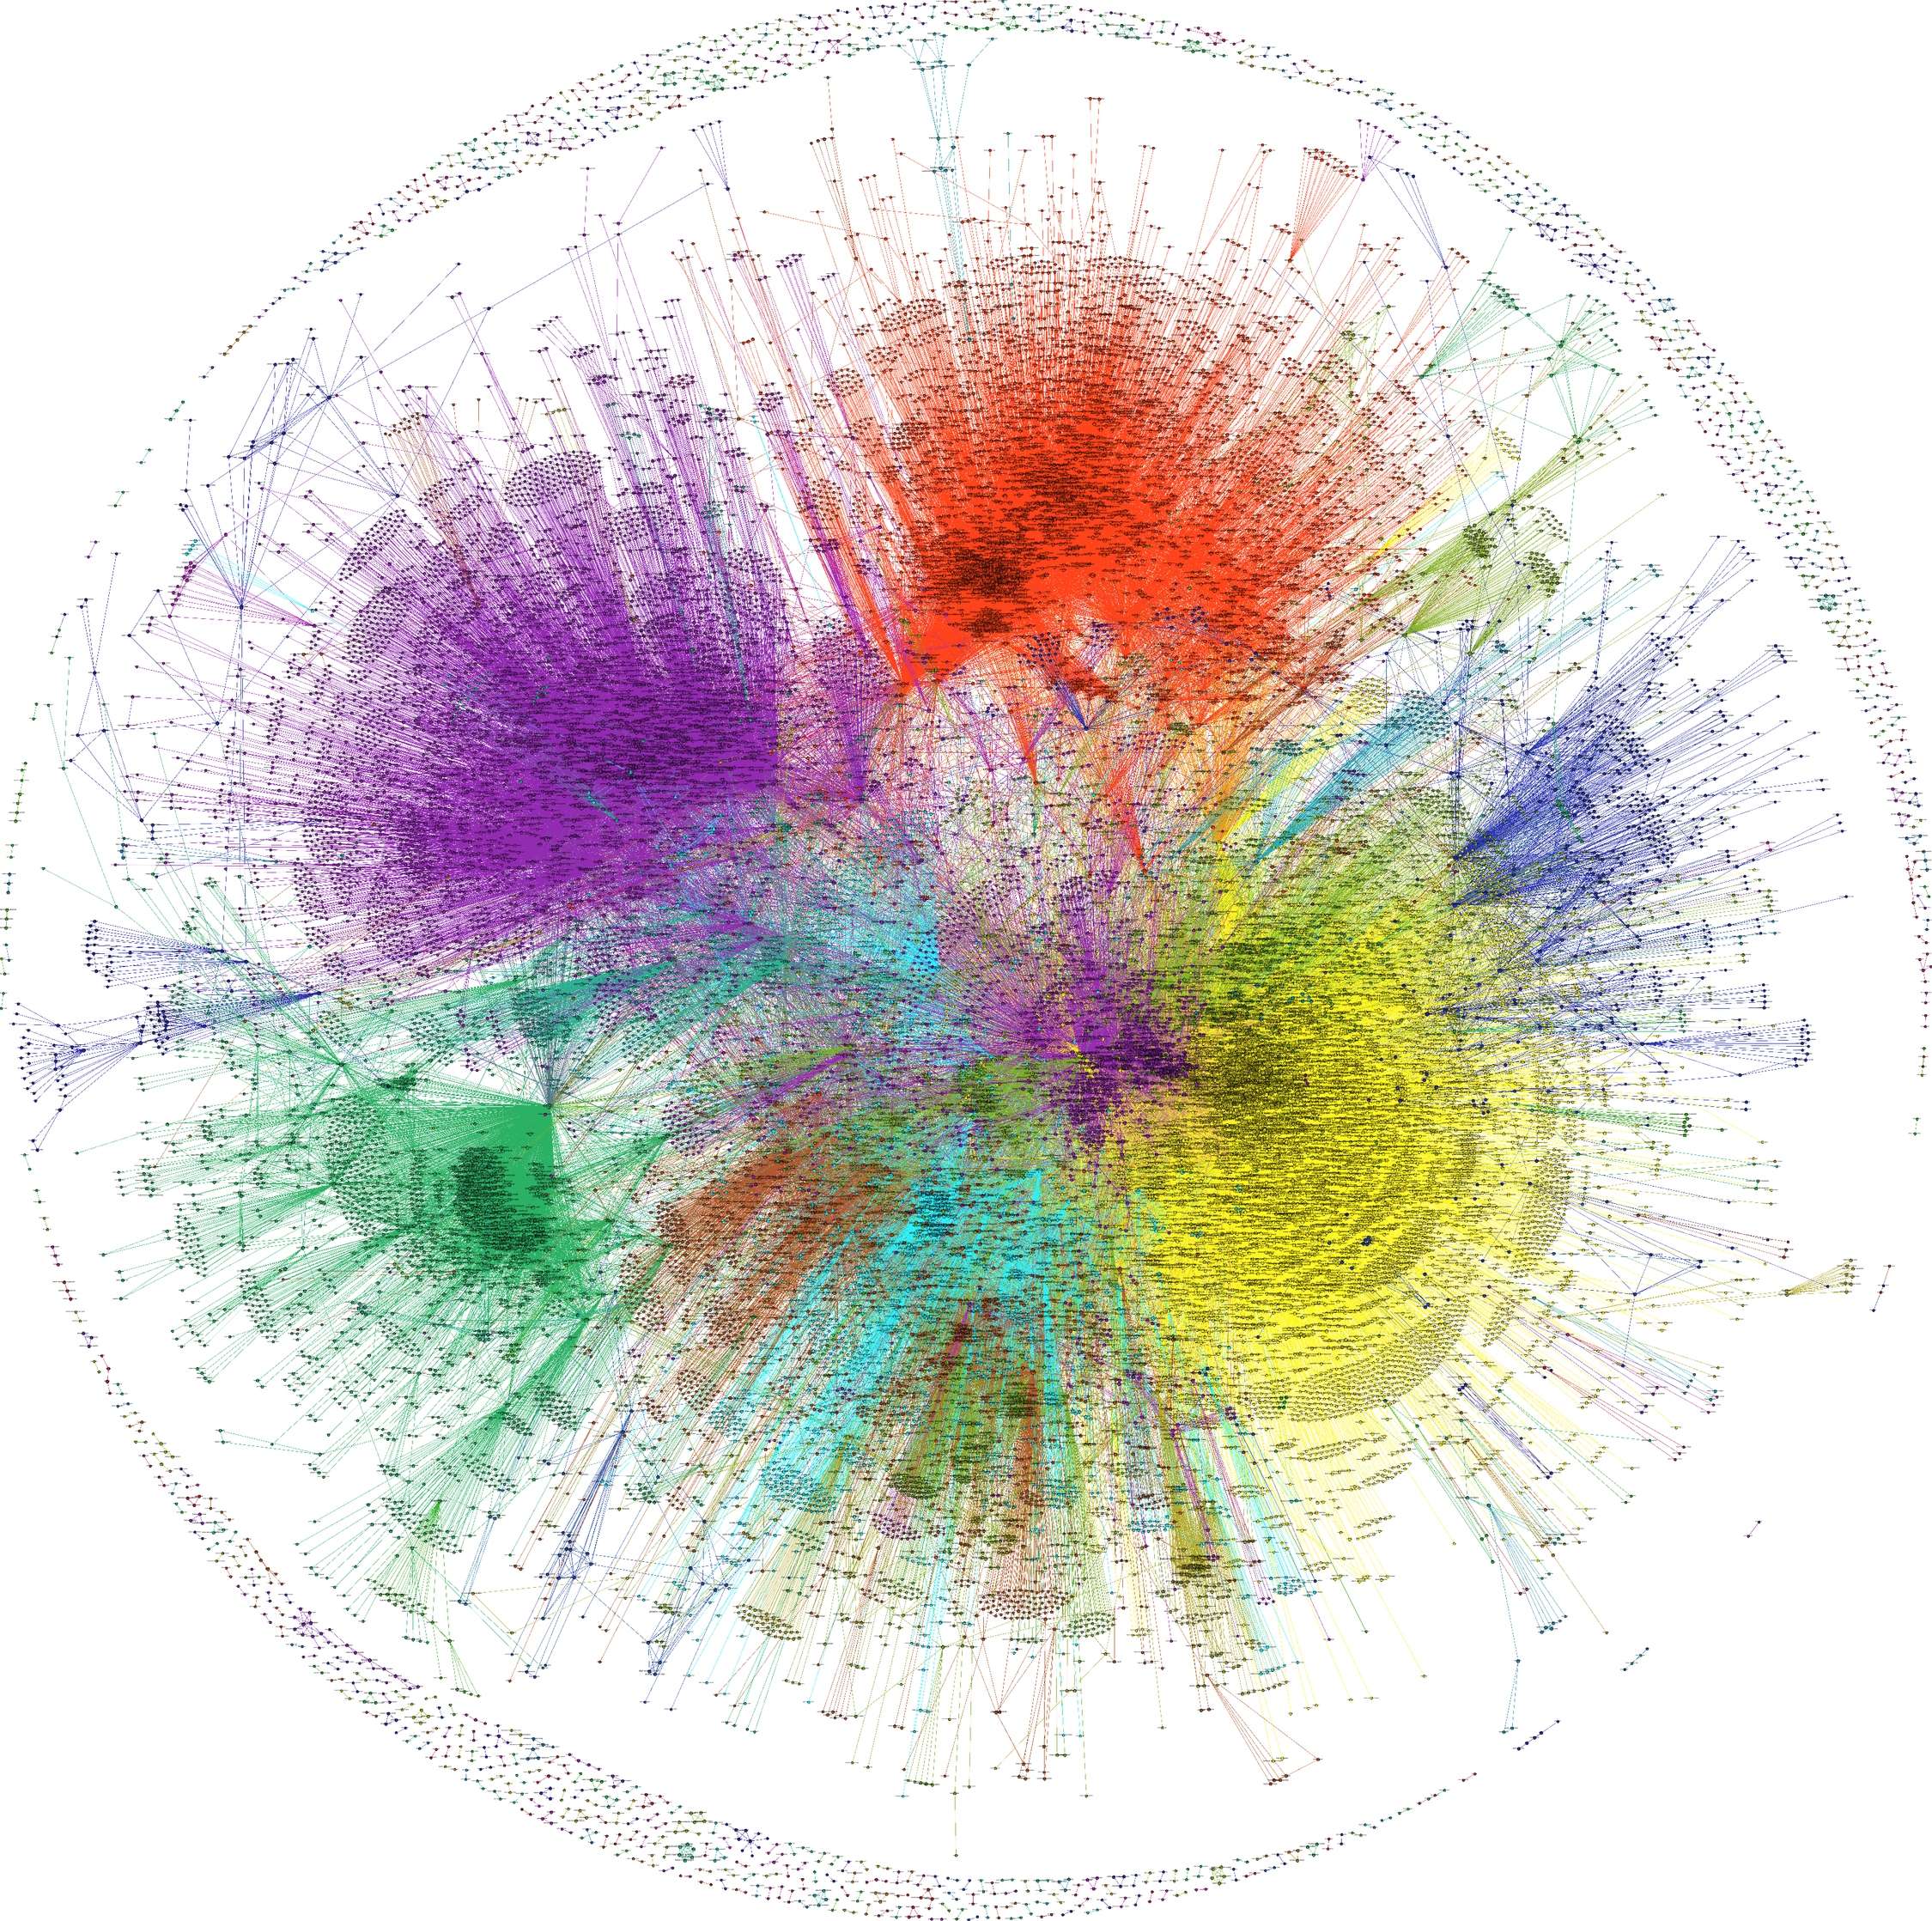
\includegraphics[width=\linewidth]{Figures/Density/Fig2}
%ex_sp-diffusion=0.05_sp-growth-rate=76_sp-diffusion-steps=2_sp-alpha-localization=0.4_ticks=995_sp-population=75620.00000000015.png
%ex_sp-diffusion=0.047_sp-growth-rate=274_sp-diffusion-steps=2_sp-alpha-localization=1.4_ticks=197_sp-population=53977.999999999935.png
%ex_sp-diffusion=0.0060_sp-growth-rate=25_sp-diffusion-steps=1_sp-alpha-localization=0.4_ticks=176_sp-population=4400.000000000003.png
%ex_sp-diffusion=0.0060_sp-growth-rate=268_sp-diffusion-steps=1_sp-alpha-localization=1.6_ticks=285_sp-population=76376.00000000033.png
\caption[Example of the variety of generated urban shapes][Exemple de formes urbaines générées]{\textbf{Example of the variety of generated urban shapes.} \textit{(Top left)} Very diffuse urban configuration, $\alpha = 0.4,\beta = 0.05, n_d = 2, N_G = 76, P_m = 75620$; \textit{(Top Right)} Semi-stationary polycentric urban configuration, $\alpha = 1.4,\beta = 0.047, n_d = 2, N_G = 274, P_m = 53977$; \textit{(Bottom Left)} Intermediate settlements (peri-urban or densely populated rural area), $\alpha = 0.4,\beta = 0.006, n_d = 1, N_G = 25, P_m = 4400$; \textit{(Bottom Right)} Rural area, $\alpha = 1.6,\beta = 0.006, n_d = 1, N_G = 268, P_m = 76376$.}{\textbf{Exemple de la variété de formes urbaines générées.} \textit{(Haut Gauche)} Configuration urbaine très diffuse, $\alpha = 0.4,\beta = 0.05, n_d = 2, N_G = 76, P_m = 75620$; \textit{(Haut Droite)} Configuration polycentrique urbaine semi-stationnaire, $\alpha = 1.4,\beta = 0.047, n_d = 2, N_G = 274, P_m = 53977$; \textit{(Bas Gauche)} Etablissements intermédiaires (périurbain ou zone rurale densément peuplée), $\alpha = 0.4,\beta = 0.006, n_d = 1, N_G = 25, P_m = 4400$; \textit{(Bas Droite)} Zone rurale, $\alpha = 1.6,\beta = 0.006, n_d = 1, N_G = 268, P_m = 76376$.}
\label{fig:density:fig2}
\end{figure}
%%%%%%%%%%%%%




%%%%%%%%%%%%%%%%%%%%%%%%
\subsubsection{Model Behavior}{Comportement du modèle}


\bpar{
In the study of such a computational model of simulation, the lack of analytical tractability must be compensated by an extensive knowledge of model behavior in the parameter space~\cite{banos2013pour}. This type of approach is typical of what Arthur calls the \emph{Computational shift in modern science}~\cite{arthur2015complexity}: knowledge is less extracted through analytical exact resolution than through intensive computational experiments, even for ``simple'' models such as the one we study.
}{
Dans l'étude d'un tel model computationnel de simulation, le manque de traçabilité analytique doit être compensé par une connaissance extensive du comportement du modèle dans l'espace des paramètres~\cite{banos2013pour}. Ce type d'approche est typique de ce qu'\noun{Arthur} nomme le \emph{tournant computationnel dans la science moderne}~\cite{arthur2015complexity} : la connaissance est moins extraite de résolutions analytiques exactes que par des expériences de calcul intensif, même pour des modèles ``simples'' comme celui que nous étudions.
}

\paragraph{Convergence}{Convergence}


\bpar{
First of all we need to assess the convergence of the model and its behavior regarding stochasticity. We run for a sparse grid of the parameter space consisting of 81 points, with 100 repetitions for each point. Corresponding histograms are shown in~\nameref{S1_Text}. Indicators show good convergence properties: most of indicators are easily statistically discernable across parameter points, and these are distinguished without ambiguity when taking into account all indicators. We use this experiment to find a reasonable number of repetitions needed in larger experiments. For each point, we estimate the Sharpe ratios for each indicators, i.e. mean normalized by standard deviation. The more variable indicator is Moran with a minimal Sharpe ratio of 0.93, but for which the first quartile is at 6.89. Other indicators have very high minimal values, all above 2. Its means than confidence intervals large as $1.5 \cdot \sigma$ are enough to differentiate between two different configurations. In the case of gaussian distribution, we know that the size of the 95\% confidence around the average is given by $2\cdot \sigma \cdot 1.96 / \sqrt{n}$, what gives $1.26 \cdot \sigma$ for $n=10$. We run therefore this number of repetitions for each parameter point in the following, what is highly enough to have statistically significant differences between average as shown above. In the following, when referring to indicator values for the simulated model, we consider the ensemble averages on these stochastic runs.
}{
Dans un premier temps il est important d'assurer la convergence du modèle et son comportement au regard de la stochasticité. Nous simulons le modèle pour une grille creuse de l'espace des paramètres contenant 81 points, avec 100 répétitions à chaque point. Les histogrammes correspondants sont montrés en Appendice~\ref{app:sec:density}. Les indicateurs présentent de bonnes propriétés de convergence: la plupart des indicateurs sont aisément discernable de manière statistique entre les points de paramètres, et ceux-ci sont distinguables sans ambiguité quand tous les indicateurs sont pris en compte. Nous utilisons cette expérience pour établir un nombre raisonnable de répétitions nécessaire pour des expériences plus volumineuses. Pour chaque point, nous estimons le ratio de Sharpe pour chaque indicateur, i.e. sa moyenne normalisée par la déviation standard. L'indicateur le plus variable est l'index de Moran avec un Sharpe minimal de 0.93, mais pour lequel le premier quartile est à 6.89. Les autres indicateurs ont tous des valeurs minimales très hautes, toutes au dessus de 2. Cela signifie que des intervalles de confiance large comme $1.5 \cdot \sigma$ sont suffisants pour différencier entre deux configurations différentes. Dans le cas d'une distribution Gaussienne, nous savons que la taille de l'intervalle de confiance à 95\% autour de la moyenne est donné par $2\cdot \sigma \cdot 1.96 / \sqrt{n}$, ce qui donne $1.26 \cdot \sigma$ pour $n=10$. Nous utilisons pour cela ce nombre de répétitions pour chaque point de paramètres par la suite, ce qui est largement suffisant pour avoir des différences entre les moyennes étant statistiquement signifiantes comme montré précédemment. Par la suite, lorsque nous considérons les valeurs des indicateurs pour le modèle simulé, nous considérons la moyenne d'ensemble sur ces répétitions stochastiques.  
}


% -> 10 repetitions give 1.24 \sigma : ok with these sharp

%       id       meanMoran            sdMoran           sharpeMoran        meanSlope      
% Min.   : 0   Min.   :0.0000997   Min.   :4.387e-05   Min.   : 0.9372   Min.   :-2.1220  
% 1st Qu.:20   1st Qu.:0.0026494   1st Qu.:3.055e-04   1st Qu.: 6.8929   1st Qu.:-1.0264  
% Median :40   Median :0.0102259   Median :1.024e-03   Median :10.0594   Median :-0.7326  
% Mean   :40   Mean   :0.0245863   Mean   :1.707e-03   Mean   :12.5250   Mean   :-0.7889  
% 3rd Qu.:60   3rd Qu.:0.0330126   3rd Qu.:2.469e-03   3rd Qu.:14.1114   3rd Qu.:-0.4594  
% Max.   :80   Max.   :0.1174664   Max.   :6.309e-03   Max.   :50.0461   Max.   :-0.1470  
%    sdSlope          sharpeSlope       meanEntropy       sdEntropy         sharpeEntropy      
% Min.   :0.001956   Min.   :  9.104   Min.   :0.2161   Min.   :4.852e-05   Min.   :    6.904  
% 1st Qu.:0.004311   1st Qu.: 17.323   1st Qu.:0.5240   1st Qu.:2.192e-04   1st Qu.:   18.503  
% Median :0.019704   Median : 40.997   Median :0.8685   Median :7.370e-03   Median :   69.986  
% Mean   :0.035573   Mean   : 57.884   Mean   :0.7529   Mean   :1.618e-02   Mean   : 3244.566  
% 3rd Qu.:0.047804   3rd Qu.: 72.753   3rd Qu.:0.9865   3rd Qu.:3.037e-02   3rd Qu.: 4479.465  
% Max.   :0.225275   Max.   :293.529   Max.   :0.9982   Max.   :5.675e-02   Max.   :20571.273  
%  meanDistance       sdDistance       sharpeDistance   
% Min.   :0.09208   Min.   :0.001579   Min.   :  1.922  
% 1st Qu.:0.44556   1st Qu.:0.002742   1st Qu.:  4.243  
% Median :0.89682   Median :0.020469   Median : 24.374  
% Mean   :0.68723   Mean   :0.050225   Mean   :152.769  
% 3rd Qu.:0.91474   3rd Qu.:0.105676   3rd Qu.:326.653  
% Max.   :0.92342   Max.   :0.182181   Max.   :579.846  





\paragraph{Exploration of parameter space}{Exploration de l'espace des paramètres}


\bpar{
We sample the Parameter space using a Latin Hypercube Sampling, with parameter as $\alpha \in [0.1,4],\beta \in [0,0.5],n_d \in \{1,\ldots , 5\}, N_G \in [500,30000], P_m \in [1e4,1e6]$. This type of cribbing is a good compromise to have a reasonable sampling without being subject to the dimensionality curse within normal computation capabilities. We sample around 80000 parameters points, with 10 repetitions each. Full plots of model behavior as a function of parameters are given in~\ref{app:sec:density}. We show in~\ref{fig:density:fig3} some particularly interesting behavior for slope $\gamma$ and average distance $\bar{d}$. First of all, the overall qualitative behavior depending on aggregation strength, namely that lower alpha giver less hierarchical and more spread configurations, confirms the expected intuitive behavior. The effect of diffusion strength $\beta$ is more difficult to grasp: the effect is inverted for slope between high and low growth rates but not for distance, that shows an inversion when $\alpha$ varies. In the low $N_G$ case, low diffusion creates more sprawled configuration when aggregation is low, but less sprawled when aggregation is high. Furthermore, all indicators show a more or less smooth transition around $\alpha \simeq 1.5$. Slope stabilize over certain values, meaning that the hierarchy cannot be forced more and indeed depends of the diffusion value, at least for low $N_G$ (right column). In general, higher valued for $P_m/N_G$ increase the effect of diffusion what could have been expected. The existence of a minimum for slope at $n_d=1,P_m/N_G\in\left[13,26\right]$ and lowest $\beta$ is unexpected and witnesses a complex interplay between aggregation and diffusion. The emergence of this ``optimal'' regime is associated with shifts of the transition points in other cases: for example, lowest diffusion imply a transition beginning at lower values of $\alpha$ for average distance. This exploration confirms that complex behavior, in the sense of unpredictable emerging forms, occurs in the model: one cannot say in advance the final form given some parameters, without referring to the full exploration of which we give an overview here.
}{
Nous échantillonnons l'espace des paramètres en utilisant un \emph{Latin Hypercube Sampling}, les paramètres variant dans $\alpha \in [0.1,4],\beta \in [0,0.5],n_d \in \{1,\ldots , 5\}, N_G \in [500,30000], P_m \in [1e4,1e6]$. Ce type de criblage est un bon compromis pour avoir un échantillonnage raisonnable sans être soumis au sort de la dimension dans des capacité de calcul normales. Nous échantillonnons autour de 80000 points, avec 10 répétitions chacun. Des graphes complets du comportement du modèle en fonction des paramètres sont donnés en~\ref{app:sec:density}. Nous montrons en Fig.~\ref{fig:density:fig3} des comportements particulièrement intéressants pour la pente $\gamma$ et la distance $\bar{d}$. Tout d'abord, le comportement qualitatif général en fonction de la force d'agrégation, c'est à dire que des valeurs faibles de $\alpha$ donnent des configurations moins hiérarchiques et plus étalées, confirme le comportement attendu intuitivement. L'effet de la force de diffusion $\beta$ est plus difficile à cerner: l'effet est inversé pour la pente entre des haut et bas taux de croissance mais pas pour la distance, qui elle présente une inversion quand $\alpha$ varie. Dans le cas où $N_G$ est faible, une diffusion faible crée des configuration plus étalée quand l'agrégation est basse, mais moins étalées quand l'agrégation est forte. De plus, tous les indicateurs présentent une transition plus ou moins abrupte autour de $\alpha \simeq 1.5$. La pente se stabilise au dessus de certaines valeurs, ce qui veut dire que la hiérarchie ne peut pas être forcée plus et dépend alors de la valeur de la diffusion, au moins pour les faibles $N_G$ (colonne de droite). En général, des valeurs fortes pour $P_m/N_G$ augmentent les effets de la diffusion ce à quoi on pouvait s'attendre. L'existence d'un minimum pour la pente à $n_d=1,P_m/N_G\in\left[13,26\right]$ et les valeurs faibles de $\beta$ est inattendue et témoigne d'une interaction complexe entre agrégation et diffusion. L'émergence de ce régime ``optimal'' est associé avec un décalage des points de transition dans les autres cas : par exemple une diffusion plus faible implique une transition commençant à des valeurs plus faible de $\alpha$ pour la distance. Cette exploration confirme qu'un comportement complexe, au sens de formes émergentes qui ne peuvent être prédites, est présent dans le modèle : il n'est pas possible de donner en avance la forme finale étant donné un jeu de paramètres, sans se référer à l'exploration complète dont nous avons donné un aperçu ici.
}



%%%%%%%%%%%%%
\begin{figure}[h!]
\includegraphics[width=\linewidth]{Figures/Density/Fig3.png}
\caption[Behavior of indicators][Comportement des indicateurs]{\textbf{Behavior of indicators.} Slope $\gamma$ (top row) and average distance $\bar{d}$ (bottom row) as a function of $\alpha$, for different bins for $\beta$ given by curve color, for particular values $n_d=1,P_m/N_G\in\left[13,26\right]$ (left column) and $n_d=4,P_m/N_G\in\left[41,78\right]$ (right column).}{\textbf{Comportement des indicateurs.} Pente $\gamma$ (ligne du haut) et distance moyenne $\bar{d}$ (ligne du bas) comme fonction de $\alpha$, pour différentes valeurs de $\beta$ données par la couleur des courbes, pour des valeurs particulières $n_d=1,P_m/N_G\in\left[13,26\right]$ (colonne de gauche) et $n_d=4,P_m/N_G\in\left[41,78\right]$ (colonne de droite).}
\label{fig:density:fig3}
\end{figure}
%%%%%%%%%%%%%






%%%%%%%%%%%%%%%%%%%%%%%%
\subsubsection{Semi-analytical Analysis}{Analyse semi-analytique}


\bpar{
Our model can be understood as a type of reaction-diffusion model, that have been widely used in other fields such as biology: similar processes were used for example by Turing in its seminal paper on morphogenesis~\cite{turing1952chemical}. An other way to formulate the model typical to these approaches is by using Partial Differential Equations. We propose to gain insights into long-time dynamics by studying them on a simplified case. We consider the system in one dimension, such that $x\in \left[0;1\right]$ with $1/\delta x$ cells of size $\delta x$. A time step is given by $\delta t$. Each cell is characterized by its population as a random variable $P(x,t)$. We work on their expected values $p(x,t) = \Eb{P(x,t)}$, and assume that $n_d=1$. As developed in Supplementary Material~\ref{app:sec:density}, we show that this simplified process verifies the following PDE:
}{
Notre modèle peut être compris comme un type de modèle de réaction-diffusion, qui ont été utilisés largement dans d'autres champs comme la biologie: des processus similaires ont par exemple été utilisés par \noun{Turing} dans son article séminal sur la morphogenèse~\cite{turing1952chemical}. Une autre façon de formuler le modèle typique à ces approches est d'utiliser des Equations aux Dérivées Partielles (PDE). Nous proposons d'éclairer des comportements des dynamiques de temps long en les étudiant sur un cas simplifié. Nous considérons le système en une dimension, tel que $x\in \left[0;1\right]$ avec $1/\delta x$ cellule de taille $\delta x$. Un pas de temps est donné par $\delta t$. Chaque cellule est caractérisée par sa population comme une variable aléatoire $P(x,t)$. Nous travaillons sur les espérances $p(x,t) = \Eb{P(x,t)}$, et supposons que $n_d=1$. Comme développé en Information Supplémentaire~\ref{app:sec:density}, on peut montrer que ce processus simplifié obéit à la PDE suivante :
}


\begin{equation}\label{eq:pde}
\hspace{-1.5cm}
\delta t \cdot \frac{\partial p}{\partial t} = \frac{N_G \cdot p^{\alpha}}{P_{\alpha}(t)} + \frac{\alpha \beta (\alpha - 1) \delta x^2}{2}\cdot \frac{N_G \cdot p^{\alpha-2}}{P_{\alpha}(t)} \cdot \left(\frac{\partial p}{\partial x}\right)^2 + \frac{\beta \delta x^2}{2} \cdot \frac{\partial^2 p}{\partial x^2} \cdot\left[ 1 + \alpha \frac{N_G p^{\alpha - 1}}{P_{\alpha(t)}} \right]
\end{equation}


\bpar{
where $P_{\alpha}(t) = \int_x p(x,t)^{\alpha} dx$. This non-linear equation can not be solved analytically, the presence of integral terms putting it out of standard methods, and numerical resolution must be used~\cite{tadmor2012review}. It is important to note that the simplified model can be expressed by a PDE analog to reaction-diffusion equations, as the one partially solved for a simpler model in~\cite{bosch1990velocity}. We show in \ref{app:sec:density} that because of the boundaries conditions, density (proportion of population) converges towards a stationary solution at long times, going through intermediate states in which the solution is partially stabilized, in the sense that its evolution speed becomes rather slow. These ``semi-stationary'' states are the ones used in two dimensions along with the dynamical ones. This study confirms that the variety of shapes obtained through the model is permitted both by the interplay of aggregation and diffusion as the equation couples them, but also by the values of $P_m / N_G$ that allow to set the convergence level. Indeed, the sensitivity of the stationary solution to parameters is very low compared to the shape of the world, and using the model in stationary mode would make no sense in our case. Finally, we use this toy case to demonstrate the importance of bifurcations in model dynamics. More precisely, we show that path-dependence is crucial for the final form. As illustrated in Fig.~\ref{fig:density:fig4}, using an initial condition making the choice ambiguous, corresponding to five equidistant equally populated cells, produces very different trajectories, as generally one of the spots will end dominating the others, but is totally random, witnessing dramatic bifurcations in the system at initial times. This aspect is typically expected in urban systems, and confirms the importance of robust indicators described before.
}{
où $P_{\alpha}(t) = \int_x p(x,t)^{\alpha} dx$. Cette équation non-linéaire ne peut pas être résolue analytiquement, la présence de termes intégraux la mettant hors des méthodes standard, et la résolution numérique doit être utilisée~\cite{tadmor2012review}. Il est important de noter que le modèle simplifié peut être exprimé comme une PDE analogue aux équations de réaction-diffusion, comme celle partiellement résolue pour un modèle plus simple dans~\cite{bosch1990velocity}. Nous montrons en \ref{app:sec:density} qu'à cause des conditions au bord, la densité (au sens de la proportion de population) converge vers une solution stationnaire sur le temps long, en passant par des états intermédiaires pour lesquels la solution est partiellement stabilisée, au sens où sa vitesse d'évolution devient relativement lente. Ces états ``semi-stationnaires'' sont ceux utilisés en deux dimensions avec les états dynamiques. Cette étude confirme que la variété des formes obtenue par le modèle est permise à la fois par l'interactions entre l'agrégation et la diffusion puisque l'équation les couple, mais aussi par les valeurs de $P_m / N_G$ qui permet de fixer le niveau de convergence. En effet, la sensibilité de la solution stationnaire aux paramètres est très faible en comparaison de la forme du monde (en écho à notre étude sur la sensibilité aux conditions spatiales initiales en~\ref{sec:computation}), et utiliser le modèle en mode stationnaire n'aurait aucun sens dans notre cas. Enfin, nous utilisons ce cas simplifié pour démontrer l'importance des bifurcations dans la dynamique du modèle. Plus précisément, nous montrons que la dépendance au chemin est cruciale pour la forme finale. Comme illustré en Fig.~\ref{fig:density:fig4}, l'utilisation d'une condition initiale rendant les choix ambigus, correspondant à 5 cellules équidistantes et de population égale, produit des trajectoires très différentes, puisqu'en général l'un des lieux finira par dominer les autres, mais est complètement aléatoire, témoignant de bifurcations cruciales dans le système aux instants initiaux. Cet aspect est typiquement attendu dans les systèmes urbains, et confirme l'importance d'indicateurs morphologiques robustes décrits précédemment.
}


%%%%%%%%%%%%%
\begin{figure}[h!]
\includegraphics[width=\linewidth]{Figures/Density/Fig4.png}
\caption[Randomness and frozen accidents][Dépendance au chemin]{\textbf{Randomness and frozen accidents.} We show nine random realizations of the one dimensional system with similar initial conditions, namely five equidistant equally populated initial cells. Parameters are $\alpha = 1.4,\beta =0.1,N_G=10$. Each plot shows time against space, color level giving the proportion of population in each cell.}{\textbf{Aléatoire et accidents figés.} Nous montrons 9 réalisations aléatoires du système à une dimension avec des conditions initiales identiques, c'est à dire 5 cellules équidistantes peuplées également à l'instant initial. Les paramètres sont $\alpha = 1.4,\beta =0.1,N_G=10$. Chaque graphe montre le temps contre l'espace, le niveau de couleur donnant la proportion de population dans chaque cellule.}
\label{fig:density:fig4}
\end{figure}
%%%%%%%%%%%%%





%%%%%%%%%%%%%%%%%%%%%%%%
\subsubsection{Model Calibration}{Calibration du modèle}


\bpar{
We finally turn to the the calibration of the model, that is done on the morphological objectives. As a single calibration for each real cell is computationally out of reach, we use the previous model exploration and superpose the point clouds with real indicator values. Full scatterplots of all indicators against each other, for simulated and real configurations, are given in~\ref{app:sec:density}. We find that the real point cloud is mostly contained within the simulated, that extend in significantly larger areas. It means that for a large majority of real configuration, there exist model parameters producing in average exactly the same morphological configuration. The highest discrepancy is for the distance indicator, the model failing to reproduce configuration with high distance, low Moran and intermediate hierarchy. These could for example correspond to polycentric configurations with many consequent centers. We consider a more loose calibration constraint, by doing a Principal Component Analysis on synthetic and real morphological values, and consider the two first components only. These represent 85\% of cumulated variance. The rotated point clouds along these dimensions are shown in Fig.~\ref{fig:density:densitycalib}. Most of real point cloud falls in the simulated one in this simplified setting. We illustrate particular points with real configurations and their simulated counterparts: for example Bucharest, Romania, corresponds to a monocentric semi-stationary configuration, with very high aggregation but also diffusion and a rather low growth rate. Other examples show less populated areas in Spain and Finland. From the plots giving parameter influence, we can show that most real situation fall in the region with intermediate $\alpha$ but quite varying $\beta$. It is consistent with real scaling urban exponents having a variation range rather small (between 0.8 and 1.3 generally~\cite{pumain2006evolutionary}) compared to the one we allowed in the simulations, whereas the diffusion processes may be much more diverse. This way, we have shown that the model is able to reproduce most of existing urban density configuration in Europe, despite its rather simplicity. It confirms that in terms of urban form, most of drivers at this scale can be translated into these abstract processes of aggregation and diffusion, but also that function must be quite correlated with form since the dimension of function (with an additional economic dimension in form for example) is not taken into account in the model.
}{
Nous traitons finalement la calibration du modèle, qui est faite sur les objectifs morphologiques. Comme une calibration pour chaque cellule réelle est hors de portée en terme de calcul, nous utilisons l'exploration précédente du modèle et superposons le nuage de points avec les valeurs réelles des indicateurs. Les scatterplots complets de chaque indicateur contre les autres, pour les configurations simulées et les réelles, sont donnés en~\ref{app:sec:density}. Nous constatons que le nuage de points réels est en majorité contenu dans le simulé, qui s'étend sur des zones significativement plus grandes. Cela signifie que pour une grande majorité des configurations réelles, il existe des valeurs des paramètres qui produisent en moyenne exactement la même configuration morphologique. Les plus grands écarts est pour l'indicateur de distance, le modèle échouant à produire des configurations avec une valeur élevée de la distance, un Moran faible et une hiérarchie intermédiaire. Cela peut par exemple correspondre à des configurations polycentriques avec de nombreux centres conséquents. Nous considérons une contrainte de calibration plus faible, en procédant à une analyse en composantes principales sur les valeurs normalisées des indicateurs morphologiques pour les configurations synthétiques et réelles, et ne considérons que les deux premières composantes seulement. Celles-ci représentent 85\% de la variance cumulée. Les nuages de points projeté sur ces dimensions est montré en Fig.~\ref{fig:density:densitycalib}. La majorité du nuage réel tombe dans le simulé dans cette configuration simplifiée. Nous illustrons des points particuliers avec des configurations réelles et leur contrepartie simulée: par exemple Bucarest, Roumanie, correspond à une configuration monocentrique semi-stationnaire, avec une forte agrégation mais aussi diffusion et un taux de croissance plutôt bas. Les autres exemples montrent des zones moins peuplées en Espagne et en Finlande. A partir des graphes montrant l'influence des paramètres, on peut montrer que la plupart des situations réelles tombent dans la région avec des valeurs intermédiaires pour $\alpha$ mais $\beta$ assez variable. Cela est cohérent avec le fait que les exposants de lois d'échelles urbaines ont une plage de variation plutôt étroite (entre 0.8 et 1.3 généralement~\cite{pumain2006evolutionary}) comparée à celle que nous avons permis dans les simulations, tandis que les processus de diffusion peuvent être bien plus divers. Ainsi, nous avons montré que le modèle est capable de reproduire la majorité des configuration de densité en Europe, malgré sa relative simplicité. Cela confirme qu'en terme de forme urbaine, la plupart des facteurs à cette échelle peuvent être traduits dans ces processus abstraits d'agrégation et de diffusion, mais aussi que la fonction doit être relativement corrélée à la forme puisque la dimension fonctionnelle (avec une dimension économique supplémentaire dans la forme par exemple) n'est pas prise en compte dans le modèle.
}


% Calib 1 :
% real : PC1 = 0.9544645 ; PC2 = 0.3296364 ; coordinates : -2.607152,39.74274 - Spain, Castilla-La Mancha, Cuenca ; synth : PC1 = 0.9487267 PC2 = 0.3245882 ; beta=0.108 ; NG=637 ; nd=1 ; alpha=1.14 ; population=13235.648362769914
% Calib 2 :
% real : PC1 = 0.7004772 ; PC2 = 0.2195029 ; coordinates : 27.16068,65.889 - Finland, Lapland;  synth :  PC1 = 0.6870686 ; PC2 = 0.2287785 ; beta=0.0060 ; NG=25 ; nd=1 ; alpha=0.4 ; population=849.895449367323
% Calib 3 :
% real : PC1 = 1.017064 ; PC2 = 0.3510089 ; coordinates : -2.561874,41.30203 - Spain, Castilla et Leon, Soria ; synth : PC1 = 1.005976 PC2 = 0.3950987 ; beta=0.166; NG=100;nd=1;alpha=1;population=10017.238452906771
% Calib 4 :
% real : PC1 = -0.00177 ; PC2 = 0.6006739 ; coordinates : 25.7361,44.69989 - Romania, Bucharest ; synth : PC1 = -0.0543461 PC2 = 0.5798307 ; beta=0.432;NG=1273;nd=4;alpha=3.87;population=63024.359885979036


%%%%%%%%%%%%%%%
\begin{figure}
\includegraphics[width=\linewidth]{Figures/Density/Fig5}
\caption[Model calibration][Calibration du modèle]{\textbf{Model calibration.} \textit{(Top)} Simulated configurations in the two first principal components plan, color level giving the influence of $\alpha$ (left) and of $\beta$ (right); \textit{(Bottom)} Simulated points in the same space (in black) with real configurations (in red). We show around the plot typical examples of real configurations and their simulated counterparts in different regions of the space, the first being the real and the second the simulated in each case: Top left geographical coordinates 25.7361,44.69989 - Romania, Bucharest - simulation parameters $\alpha=3.87,\beta=0.432,N_G=1273,nd=4,P_m=63024$ ; Top right geographical coordinates -2.561874,41.30203 - Spain, Castilla et Leon, Soria - simulation parameters $\alpha=1,\beta=0.166,N_G=100,nd=1,P_m=10017$; Bottom left geographical coordinates 27.16068,65.889 - Finland, Lapland - simulation parameters $\alpha=0.4,\beta=0.006,N_G=25,nd=1,P_m=849$; Bottom right geographical coordinates -2.607152,39.74274 - Spain, Castilla-La Mancha, Cuenca - simulation parameters $\alpha=1.14,\beta=0.108,N_G=637,nd=1,P_m=13235$.}{\textbf{Calibration du modèle.} \textit{(Haut)} Configurations simulées dans le plan des deux premières composantes principales, le niveau de couleur donnant l'influence de $\alpha$ (gauche) et de $\beta$ (droite); \textit{(Bas)} Points simulés dans le même espace (en noir) avec les configurations réelles (en rouge). Autour du graphe sont montrés des exemples typiques de configurations réelles et leur contrepartie simulée dans différentes régions de l'espace, le premier étant le réel et le second le simulé dans chaque cas: haut gauche coordonnées 25.7361,44.69989 - Romania, Bucharest - paramètres $\alpha=3.87,\beta=0.432,N_G=1273,nd=4,P_m=63024$ ; Haut droite coordonnées -2.561874,41.30203 - Spain, Castilla et Leon, Soria - paramètres $\alpha=1,\beta=0.166,N_G=100,nd=1,P_m=10017$; Bas gauche coordonnées 27.16068,65.889 - Finland, Lapland - paramètres $\alpha=0.4,\beta=0.006,N_G=25,nd=1,P_m=849$; Bas droite coordonnées -2.607152,39.74274 - Spain, Castilla-La Mancha, Cuenca - paramètres $\alpha=1.14,\beta=0.108,N_G=637,nd=1,P_m=13235$.}
\label{fig:densitycalib}
\end{figure}
%%%%%%%%%%%%%%








%%%%%%%%%%%%%%
\subsection{Discussion}{Discussion}




\paragraph{Calibration and model refinement}{Raffinement de la calibration et du modèle}


\bpar{
Further work on this simple model may consist in extracting the exact parameter space covering all real situations and provide interpretation of its shape, in particular through correlations between parameters and expressions of boundaries functions. Its volume in different directions should furthermore give the relative importance of parameters. Concerning the feasible space for the model of simulation itself, we tested a targeted exploration algorithm, giving promising results. More precisely, the Parameter Space Exploration (PSE) algorithm~\cite{10.1371/journal.pone.0138212} which is implemented in OpenMole, is aimed at determining all the possible outputs of a simulation model, i.e. samples its output space rather than input space. We obtain promising results as shown in Fig.~\ref{fig:fig6}: we find that the lower bound in Moran-entropy plan, confirmed by the algorithm, unexpectedly exhibit a scaling relationship. It would mean that at a given level of auto-correlation, that one could want to attain for sustainability reasons for example (optimality through co-location), imposes a minimal disorder in the configuration of activities. Other relations between indicators and as a function of parameters can be the object of similar future developments. The question of doing a dynamical calibration of the model, i.e. trying to reproduce configurations at successive times, is conditioned to the availability of population data at this resolution in time.
}{
Des développements futurs sur ce modèle simple peuvent consister à l'extraction de l'espace des paramètres exact couvrant l'ensemble des situations réelles et fournir une interprétation de sa forme, en particulier par les corrélations entre les paramètres et les expressions des fonctions de bordure. Son volume dans différentes directions devrait de plus donner l'importance relative des paramètres. Concernant l'espace faisable pour le modèle de simulation en lui-même, nous avons testé un algorithme d'exploration ciblée, qui donne des résultats prometteurs. Plus précisément, l'algorithme PSE~\cite{10.1371/journal.pone.0138212} qui est implémenté dans OpenMole, a pour but de déterminer toutes les sorties possibles d'un modèle de simulation, c'est à dire échantillonne son espace de sortie plutôt que d'entrée. Nous obtenons des résultats intéressants comme montré en Fig.~\ref{fig:density:fig6}: nous trouvons que la borne inférieure dans le plan Moran-entropie, confirmée par l'algorithme, exhibe une loi d'échelle de manière inattendue (puisqu'il est impossible a priori de déterminer cet espace non-faisable avec seule les formules des d'indicateurs, celui-ci étant témoin de la réalité de structures urbaines même simulées). Cela voudrait dire qu'à un niveau fixé d'auto-corrélation, qu'on pourrait vouloir atteindre pour des raisons de soutenabilité par exemple (optimalité par co-localisation), impose un désordre minimal dans la configuration des activités. D'autres relations entre indicateurs et comme fonction des paramètres peut être l'objet de développements futurs similaires. La possibilité d'une calibration dynamique du modèle, i.e. essayer de reproduire des configurations à des dates successives, est conditionnée à la disponibilité des données de population à cette résolution dans le temps.
}

% application of Calibration Profile algo to check relative influence of parameters ? out of context not interesting

%%%%%%%%%%%%%
\begin{figure}[h!]
\includegraphics[width=\linewidth]{Figures/Density/Fig6.png}
\caption[PSE exploration][Exploration par PSE]{\textbf{PSE exploration.} Scatterplot of Moran against Entropy, with blue points obtained with LHS and red with PSE exploration. Green dashed line gives feasible lower bound.}{\textbf{Exploration par PSE.} Scatterplot de l'entropie en fonction de Moran, les points bleus étant obtenus par LHS et les rouges par PSE. La ligne pointillée verte donne la borne inférieur faisable.}
\label{fig:density:fig6}
\end{figure}
%%%%%%%%%%%%%


\bpar{
We aimed at using abstract processes rather than having a highly realistic model. Tuning some mechanisms is possible to have a model closer to reality in microscopic processes: for example thresholding the local population density, or stopping the diffusion at a given distance from the center if it is well defined. It is however far from clear if these would produce such a variety of forms and could be calibrated in a similar way, as being accurate locally does not mean being accurate at the mesoscopic level for morphological indicators. Allowing the parameters to locally vary, i.e. being non stationary in space, or adding randomness to the diffusion process, are also potential model refinements.
}{
Nous avons visé à utiliser des processus abstraits plutôt que d'avoir un modèle hautement réaliste. La modification de certains mécanismes est possible pour avoir un modèle plus proche de la réalité des processus microscopiques: par exemple plafonner la densité de population locale, ou stopper la diffusion à une distance donnée du centre s'il est bien défini. Il est cependant loin d'être clair si ceux-ci produiraient une telle variété de formes et pourraient être calibrés de la même façon, puisqu'être précis localement n'implique pas d'être précis au niveau mesoscopique pour les indicateurs morphologiques. Permettre aux paramètres de varier localement, i.e. être non-stationnaires dans l'espace, ou ajouter de l'aléatoire au processus de diffusion, sont également des raffinements potentiels du modèle.
}


\paragraph{Integration into a multi-scale growth model}{Intégration dans un modèle de croissance multi-scalaire}

\bpar{
The question of the generic character of the model is also open: would it work as well when trying to reproduce Urban Forms on very different systems such as the United States or China. A first interesting development would be to test it on these systems and at slightly different scales (1km cell for example). Finally, we believe that a significant insight into the non-stationarity of Urban Systems would be allowed by its integration into a multi-scale growth model. Urban growth patterns have been empirically shown to exhibit multi-scale behavior~\cite{zhang2013identifying}. Here at the meso-scale, total population and growth rates are fixed by exogenous conditions of processes occurring at the macro-scale. It is particularly the aim of spatial growth models such as the Favaro-pumain model~\cite{favaro2011gibrat} to determine such parameters through relations between cities as agents. One would condition the morphological development in each area to the values of the parameters determined at the level above. In that setting, one must be careful of the role of the bottom-up feedback: would the emerging urban form influence the macroscopic behavior in its turn ? Such multi-scale complex model are promising but must be considered carefully.
}{
La question du caractère générique du modèle est également ouverte, c'est à dire s'il fonctionnerait de la même manière pour reproduire des formes urbaines sur des systèmes très différents comme les Etats-Unis ou la Chine. Un premier développement intéressant serait de le tester sur ces systèmes et à des échelles légèrement différentes (cellules de taille 1km par exemple). Enfin, nous pensons qu'un gain de connaissance important concernant la non-stationnarité des systèmes urbains serait rendu possible par son intégration dans un modèle de croissance multi-échelles. Les motifs de croissance urbaine ont été prouvés empiriquement exhibant un comportement multi-échelle~\cite{zhang2013identifying}. Ici à l'échelle mesoscopique, la population totale et le taux de croissance sont fixés par les conditions exogènes de processus se produisant à l'échelle macroscopique. C'est particulièrement le but des modèles spatiaux de croissance comme le modèle Favaro-Pumain~\cite{favaro2011gibrat} de déterminer de tels paramètres par les relations entre villes comme agents. On pourrait conditionner le développement morphologique de chaque zone aux valeurs des paramètres déterminés au niveau supérieur. Dans ce contexte, il faudrait être prudent sur le rôle de la retroaction bottom-up: la forme urbaine émergente devrait-elle influence le comportement macroscopique à son tour ? De tels modèles complexes multi-scalaires sont prometteurs mais doivent être considérés avec précaution.
}


%  determination of effective independent dimensions of the urban system at this scale ?


\bpar{
In conclusion, we have provided a calibrated spatial urban morphogenesis model at the mesoscopic scale that can reproduce any European urban pattern in terms of morphology. We demonstrate that the abstract processes of aggregation and diffusion are sufficient to capture urban growth processes at this scale. It is meaningful in terms of policies based on urban form such as energy efficiency, but also means that issues out of this scope must be tackled at other scales or through other dimensions of urban systems.
}{
En conclusion, nous avons produit un modèle spatial de morphogenèse urbaine à l'échelle mesoscopique, dont la calibration permet de reproduire n'importe quelle configuration urbaine Européenne en terme de morphologie. Nous démontrons que les processus abstraits d'agrégation et diffusion sont suffisants pour capturer la dimension morphologique des processus de croissance urbaine à cette échelle. Cela a des implications par exemple en terme de politiques basées sur la forme urbaine comme l'efficacité énergétique, mais aussi signifie que les questions hors de ce cadre doivent être traitées à d'autres échelles ou par d'autres dimensions des systèmes urbains.
}





\stars











